% questions.tex —— 1977 年·江苏盐城地区初试卷 · 题目内容片段（无答案）
% 由 tools/generate_projects.py 依来源总账自 1977/1977_数学真题_江苏盐城地区初试_试题.md 生成，勿手改（改源 MD 后重跑）


\gkpart{江苏盐城地区初试卷}

\begin{gktip}
\textbf{来源说明}：本题面依据固定源 PDF《1977江苏盐城地区初试》第 1—2 页逐题转录；第 1 页原书页码 244，第 2 页无页码。源页为试题汇编材料中的盐城地区初试（预选）卷，仅题面、无解答；页首标题「九、盐城地区」系汇编章节标题，按原卷逐字保留为本文 H1。原卷大题以中文数字「一、」至「八、」编号，本库转写为 \textbf{1．}至 \textbf{8．}；第 1、2 题各设两小问并逐问标注分值，第 3、4 题为单一大题、分值印在题末，本文按本库规范移至题号后；第 5—8 题原卷未印分值，按原卷照录不补。第 4、7 题原卷附图，LaTeX 版按源图重绘。第 6 题证明式右端印作等号后接一整条分数线，未见独立负号（经局部重渲比对、并用等比数列条件代入原式复算验证），本文按确认结果转录为正值分数。原卷无附加题/参考题；配套答案与解析为本库编者独立推导，\textbf{非官方标准答案}。
\end{gktip}

\par\medskip

\begin{question}
\gkti{1}计算：

（1） $(-1)^3-\left[\left(-\dfrac12\right)^2+4^{-\frac12}\right]\div\left(\dfrac23\right)^{-2}+\left(\dfrac29\right)^0$；（7 分）

（2） $\log_2\dfrac12+\log_3\sqrt3+\lg0.01+\lg100$。（7 分）

\end{question}
\begin{question}
\gkti{2}已知：函数 $y=\sqrt{12-x}+\sqrt{2x+10}$，

（1） 求自变量 $x$ 的取值范围；（5 分）

（2） 求当 $x=4$ 时，函数 $y$ 的值。（5 分）

\end{question}
\begin{question}
\gkti{3}\textbf{（8 分）} $m$ 为何值时，方程 $x^2-2x+m=0$，有两个相等的实数根？并求出它的根。

\Needspace{0.4\textheight}
\end{question}
\begin{question}
\gkti{4}\textbf{（12 分）} 从 $\odot O$ 外一点 $A$ 作 $\odot O$ 的两条切线 $AC\text{、}AD$，$C\text{、}D$ 为切点，连接 $CO$ 并延长交 $AD$ 的延长线于 $B$，若 $AD=4\,\mathrm{cm}$，$DB=5\,\mathrm{cm}$，求 $\odot O$ 的面积。（$\pi$ 不必取近似值）
\nopagebreak[4]
\begin{center}% 1977 年江苏盐城地区初试卷第四题：圆 O 外一点 A 作两条切线 AC、AD，
% C、D 为切点，连接 CO 并延长交 AD 延长线于 B（按源卷第 1 页布局：C 在圆左上方，D、B 在下方切线上）
% 坐标推算：A=(0,0)，D=(4,0)，B=(9,0)（AD=4，DB=5）；由 C、O、B 共线与 OD⊥AB 解得
% 半径 r=sqrt(80/13)≈2.481，O=(4,2.481)，C≈(1.778,3.583)
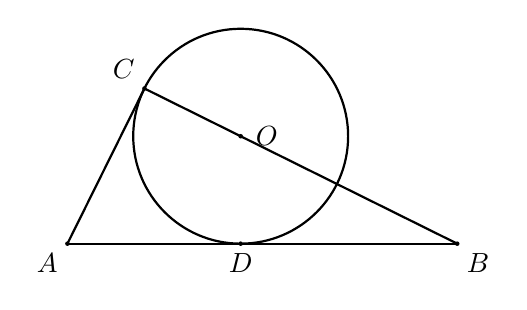
\begin{tikzpicture}[scale=0.55]
  \coordinate (A) at (0,0);
  \coordinate (D) at (4,0);
  \coordinate (B) at (9,0);
  \coordinate (O) at (4,2.481);
  \coordinate (C) at (1.778,3.583);
  \draw[thick] (O) circle (2.481);
  \draw[thick] (A) -- (B);
  \draw[thick] (A) -- (C);
  \draw[thick] (C) -- (B);
  \fill (O) circle (1.5pt) node[right=2pt] {$O$};
  \fill (A) circle (1.5pt) node[below left] {$A$};
  \fill (D) circle (1.5pt) node[below] {$D$};
  \fill (B) circle (1.5pt) node[below right] {$B$};
  \fill (C) circle (1.5pt) node[above left] {$C$};
\end{tikzpicture}
\end{center}
\nopagebreak[4]
\end{question}
\begin{question}
\gkti{5}求以双曲线 $3x^2-2y^2=6$ 的顶点为焦点，焦点为顶点的椭圆的方程。

\end{question}
\begin{question}
\gkti{6}若 $\sin\alpha\text{，}\cos\alpha\text{，}\operatorname{tg}\alpha$ 成等比数列，求证：

\nopagebreak[4]
\[
(\sin\alpha+\cos\alpha+\operatorname{tg}\alpha)(\sin\alpha-\cos\alpha+\operatorname{tg}\alpha)=\frac1{\cos^2\alpha}.
\]

\Needspace{0.4\textheight}
\end{question}
\begin{question}
\gkti{7}在边长为 $1$ 的正方形 $ABCD$ 内，作内接正方形 $A_1B_1C_1D_1$，

（1） 在什么情况下，正方形 $A_1B_1C_1D_1$ 的面积最小？最小值是多少？

（2） 在正方形 $A_1B_1C_1D_1$ 内，再作面积最小的内接正方形 $A_2B_2C_2D_2$，……，如果继续下去，求第 $n$ 个面积最小的内接正方形的面积。

（3） 这样无限制地作下去，可以得到一系列的内接正方形，求它们的面积之和。
\nopagebreak[4]
\begin{center}% 1977 年江苏盐城地区初试卷第七题：边长为 1 的正方形 ABCD 内作内接正方形 A1B1C1D1
% （按源卷第 2 页布局：A 左上、D 右上、C 右下、B 左下；A1 靠近 A、B1 靠近 B、C1 靠近 C、D1 靠近 D，图示取一般位置，非最小面积的特解）
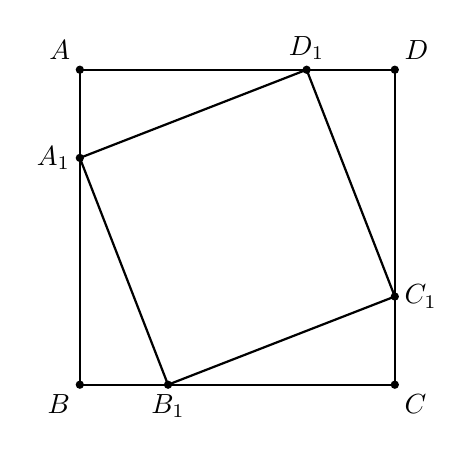
\begin{tikzpicture}[scale=1]
  \coordinate (A) at (0,4);
  \coordinate (B) at (0,0);
  \coordinate (C) at (4,0);
  \coordinate (D) at (4,4);
  \coordinate (A1) at (0,2.88);
  \coordinate (B1) at (1.12,0);
  \coordinate (C1) at (4,1.12);
  \coordinate (D1) at (2.88,4);
  \draw[thick] (A) -- (B) -- (C) -- (D) -- cycle;
  \draw[thick] (A1) -- (B1) -- (C1) -- (D1) -- cycle;
  \fill (A) circle (1.5pt) node[above left] {$A$};
  \fill (B) circle (1.5pt) node[below left] {$B$};
  \fill (C) circle (1.5pt) node[below right] {$C$};
  \fill (D) circle (1.5pt) node[above right] {$D$};
  \fill (A1) circle (1.5pt) node[left] {$A_1$};
  \fill (B1) circle (1.5pt) node[below] {$B_1$};
  \fill (C1) circle (1.5pt) node[right] {$C_1$};
  \fill (D1) circle (1.5pt) node[above] {$D_1$};
\end{tikzpicture}
\end{center}
\nopagebreak[4]
\end{question}
\begin{question}
\gkti{8}在 $\triangle ABC$ 中，最大角是最小角 $C$ 的二倍，其三边 $a\text{，}b\text{，}c$ 成等差数列，求证：这个三角形是锐角三角形。

\end{question}